\section{Zusammenfassung und Ausblick}\label{sec:08_05_zusammenfassung}
Durch die unterschiedlichen angewandten Methoden und die verwendeten Frameworks und Bibliotheken konnten wir viel Neues kennen lernen. Rückblickend konnten wir in diesem Semester eine solide und gut vorzeigbare Benutzeroberfläche für unser Informationssystem schaffen. Wir haben sehr viel positives Feedback erhalten und bei der Live-Demo und in den vorangegangenen Präsentationen hat die Webseite wie geplant funktioniert.

\begin{figure}[hbt!]
    \centering
    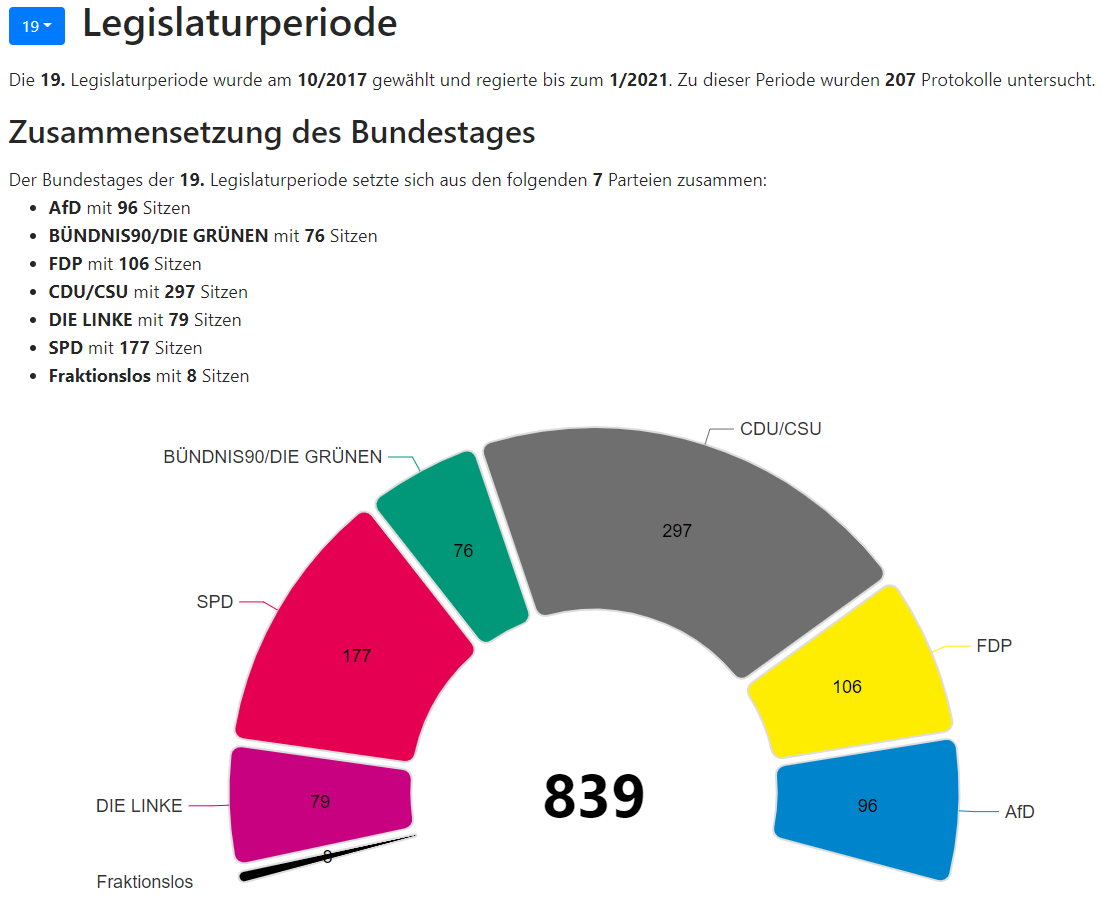
\includegraphics[width=14cm]{images/08-Benutzeroberfläche/08-Legislaturperioden.PNG}
    \caption{Screenshot aus der Benutzeroberfläche}
\end{figure}

Ein Aspekt den wir zu Beginn des Semesters unterschätzt haben war die Abhängigkeit von den vorangehenden Gruppen. Diese führte zu Zeitproblemen, Koordinationsaufwand und Problemen bei der Entwicklung. Diese Herausforderungen konnten wir nur im Team durch Zusammenarbeit und durch direkte Kommunikation mit den anderen Gruppen lösen.
Alles in Allem sind wir mit dem Projekt sehr Zufrieden. Sowohl der Lernerfolg in diesem Semester als auch das dabei entstandenen Produkt sind überzeugend. Wir hoffen sehr, dass das Projekt in Zukunft fortgeführt wird und andere Studierende den Design Thinking Prozess und die Entwicklung fortführen.

\subsection{Erreichbarkeit}
Die Webseite kann, für derzeit unbestimmte Zeit, unter http://infosys7.f4.htw-berlin.de/ erreicht werden. Sollte dieser Link nicht mehr erreichbar sein, bitte wenden Sie sich an Prof. Dr. rer. nat. Thomas Hoppe.


